\documentclass[12pt,letterpaper]{article}
\usepackage{graphicx,textcomp}
\usepackage{setspace}
\usepackage{fullpage}
\usepackage{color}
\usepackage[reqno]{amsmath}
\usepackage{amsthm}
\usepackage{fancyvrb}
\usepackage{amssymb,enumerate}
\usepackage[all]{xy}
\usepackage{endnotes}
\usepackage{lscape}
\newtheorem{com}{Comment}
\usepackage{float}
\usepackage{hyperref}
\newtheorem{lem} {Lemma}
\newtheorem{prop}{Proposition}
\newtheorem{thm}{Theorem}
\newtheorem{defn}{Definition}
\newtheorem{cor}{Corollary}
\newtheorem{obs}{Observation}
\usepackage[compact]{titlesec}
\usepackage{dcolumn}
\usepackage{tikz}
\usetikzlibrary{arrows}
\usepackage{multirow}
\usepackage{xcolor}
\newcolumntype{.}{D{.}{.}{-1}}
\newcolumntype{d}[1]{D{.}{.}{#1}}
\definecolor{light-gray}{gray}{0.65}
\usepackage{url}
\usepackage{listings}
\usepackage{color}
\usepackage{amsbsy}
\usepackage{natbib}

\definecolor{codegreen}{rgb}{0,0.6,0}
\definecolor{codegray}{rgb}{0.5,0.5,0.5}
\definecolor{codepurple}{rgb}{0.58,0,0.82}
\definecolor{backcolour}{rgb}{0.95,0.95,0.92}

\lstdefinestyle{mystyle}{
	backgroundcolor=\color{backcolour},   
	commentstyle=\color{codegreen},
	keywordstyle=\color{magenta},
	numberstyle=\tiny\color{codegray},
	stringstyle=\color{codepurple},
	basicstyle=\footnotesize,
	breakatwhitespace=false,         
	breaklines=true,                 
	captionpos=b,                    
	keepspaces=true,                 
	numbers=left,                    
	numbersep=5pt,                  
	showspaces=false,                
	showstringspaces=false,
	showtabs=false,                  
	tabsize=2
}
\lstset{style=mystyle}
\newcommand{\Sref}[1]{Section~\ref{#1}}
\newtheorem{hyp}{Hypothesis}

\begin{document}
	
	\begin{tikzpicture}[overlay, remember picture]
		\path (current page.north west) ++(1.5,-1.25) node[below right] {\textbf{FTL/IAC BMI Report}};
		\path (current page.north west) ++(1.5,-2) node[below right] {September 13, 2021};
	\end{tikzpicture}

\lstinputlisting[language=R, firstline=4416, lastline=4442]{TIAS.R}  	
\begin{figure}[H]
	\centering
	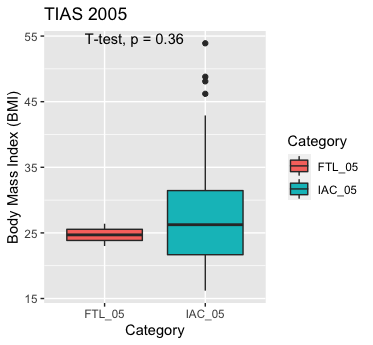
\includegraphics[scale=0.5]{bmi_boxplot_05.png}
\end{figure}			

\lstinputlisting[language=R, firstline=8709, lastline=8735]{TIAS.R}  
\begin{figure}[H]
	\centering
	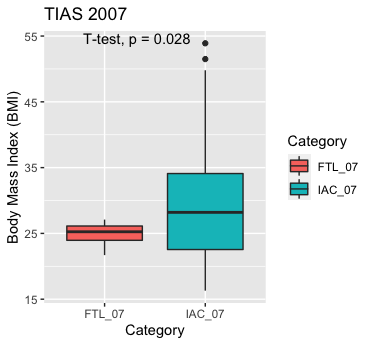
\includegraphics[scale=0.5]{bmi_boxplot_07.png}
\end{figure}	
	
\lstinputlisting[language=R, firstline=13501, lastline=13527]{TIAS.R}  
\begin{figure}[H]
	\centering
	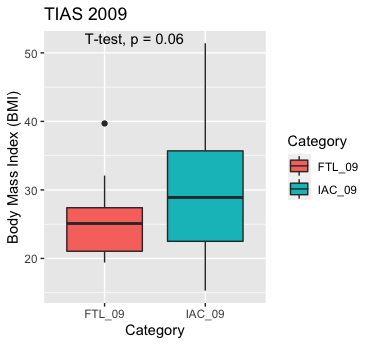
\includegraphics[scale=0.5]{bmi_boxplot_09.png}
\end{figure}		

\lstinputlisting[language=R, firstline=15774, lastline=15800]{TIAS.R}  
\begin{figure}[H]
	\centering
	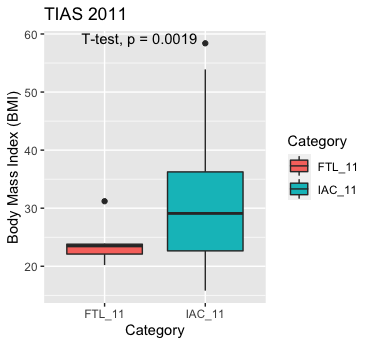
\includegraphics[scale=0.5]{bmi_boxplot_11.png}
\end{figure}		

\lstinputlisting[language=R, firstline=20926, lastline=20952]{TIAS.R}  
\begin{figure}[H]
	\centering
	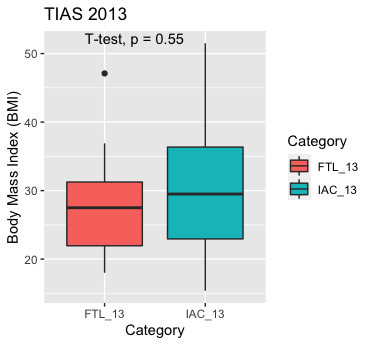
\includegraphics[scale=0.5]{bmi_boxplot_13.png}
\end{figure}	
	
\lstinputlisting[language=R, firstline=26428, lastline=26454]{TIAS.R}  
\begin{figure}[H]
	\centering
	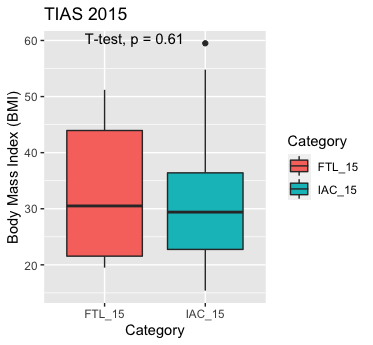
\includegraphics[scale=0.5]{bmi_boxplot_15.png}
\end{figure}	
	
\lstinputlisting[language=R, firstline=30521, lastline=30547]{TIAS.R}  
\begin{figure}[H]
	\centering
	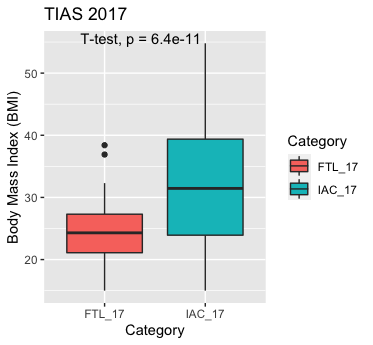
\includegraphics[scale=0.5]{bmi_boxplot_17.png}
\end{figure}		

\end{document}